% partes/parte1/cap04.tex
\chapter{Base tecnológica: buscadores, plataformas, redes y comercio electrónico}
\label{cap:04}

\section*{Ficha del capítulo}
\begin{description}
  \item[Unidad temática] I — Comportamiento, perfil y gestión de datos del consumidor digital.
  \item[Temas del programa] 1.4 Base tecnológica para la gestión de datos de los consumidores digitales: 1.4.1 Temas selectos de buscadores y plataformas de gestión integral, redes sociales y comercio electrónico.
  \item[Horas] Teoría 2.0 · Práctica 3.0 · Aprendizaje autónomo 1.0.
  \item[Competencia de la unidad] Identifica el comportamiento del consumidor digital y su evolución a partir de sus tipos de perfil y gestión de datos.
  \item[Resultados de aprendizaje observables] Al concluir el capítulo, el estudiante:
  \begin{enumerate}
    \item aplica una matriz de criterios durables para evaluar cualquier plataforma digital, presente o futura;
    \item interpreta una serie de interés de búsqueda en sus componentes de tendencia y estacionalidad;
    \item extrae y analiza frecuencia de términos de un corpus de escucha social.
  \end{enumerate}
  \item[Prerrequisitos] Cap. 1--3.
\end{description}

\section{Caso de apertura}

\textbf{Vigente a septiembre de 2026.} En 2020, buena parte del material de
mercadotecnia digital advertía que las cookies de terceros desaparecerían de
Chrome en un plazo de dos o tres años. No ocurrió (Cap.~3, §2.4). En 2024,
Gartner predijo que el volumen de búsqueda tradicional caería 25\,\% para
2026 por efecto de los chatbots de IA. Al cierre de este libro, las propias
fuentes de industria se contradicen sobre si esa caída ocurrió tal cual se
predijo. Este capítulo parte de una premisa incómoda pero honesta: cualquier
cifra puntual de cuota de mercado o de adopción tecnológica que aparezca
aquí puede estar desactualizada antes de que el estudiante egrese. Por eso
el capítulo no enseña un catálogo de plataformas —enseña los criterios para
evaluar cualquier plataforma, presente o futura, sin depender de que ninguna
marca en particular siga existiendo.

\section{Desarrollo teórico}

\subsection{Temas selectos de buscadores y plataformas: una matriz de criterios durables}
\progtag{1.4.1}

El programa oficial deja este subtema deliberadamente abierto
—\enquote{temas selectos}— precisamente porque el panorama tecnológico cambia
más rápido que cualquier edición impresa de un libro de texto. La respuesta
de este capítulo no es listar herramientas vigentes hoy (que envejecerán),
sino ofrecer cuatro criterios de análisis que se sostienen con independencia
de qué marca domine el mercado en el momento en que se lean
(figura~\ref{fig:cap04-criterios}).

\begin{figure}[htbp]
  \centering
  % figuras/tikz/cap04-criterios-evaluacion.tex
% Matriz de criterios de evaluación de plataformas digitales, diseñada para
% sobrevivir al cambio de marcas concretas (§5.7 del prompt de proyecto).
\begin{tikzpicture}[
    criterio/.style={rectangle, rounded corners, draw=guindaIPN, thick, fill=guindaIPNClara,
                     minimum width=5.6cm, minimum height=1.15cm, align=left, font=\scriptsize},
  ]
  \node[criterio] (c1) at (0,3.3)  {\textbf{Modelo de negocio}\\ publicidad / suscripción / comisión transaccional};
  \node[criterio] (c2) at (0,1.9)  {\textbf{Intermediación de datos}\\ ¿quién controla el dato del consumidor?};
  \node[criterio] (c3) at (0,0.5)  {\textbf{Interoperabilidad}\\ APIs abiertas vs. cerradas};
  \node[criterio] (c4) at (0,-0.9) {\textbf{Exposición regulatoria}\\ DSA europea, LFPDPPP mexicana};

  \node[font=\small\bfseries, align=center, text width=3.2cm] at (5.2,1.2)
    {Evaluar cualquier\\ plataforma o\\ herramienta\\ vigente con estos\\ cuatro criterios};
  \draw[-{Stealth[length=3mm]}, thick, draw=doradoIPN] (3.0,1.2) -- (3.9,1.2);
\end{tikzpicture}

  \caption{Matriz de criterios durables para evaluar buscadores, plataformas
  y redes sociales, con independencia de la marca vigente. Fuente:
  elaboración propia.}
  \label{fig:cap04-criterios}
\end{figure}

El cuadro~\ref{tab:cap04-criterios} desarrolla cada criterio con la pregunta
concreta que un mercadólogo digital debería hacerse frente a cualquier
plataforma —la que use hoy, o la que la reemplace mañana—.

\begin{table}[htbp]
\centering
\begin{tabular}{@{}p{3.3cm}p{9.1cm}@{}}
\toprule
Criterio & Pregunta de evaluación \\
\midrule
Modelo de negocio & ¿La plataforma se financia por publicidad, suscripción o comisión transaccional? Cada modelo alinea sus incentivos de forma distinta con los intereses del consumidor. \\
Intermediación de datos & ¿Quién es dueño del dato de comportamiento del consumidor generado en la plataforma: la organización que anuncia, la plataforma, o ambas bajo condiciones específicas? \\
Interoperabilidad & ¿La plataforma ofrece APIs abiertas que permiten exportar datos propios, o mantiene los datos cautivos dentro de su ecosistema cerrado? \\
Exposición regulatoria & ¿Qué marco normativo aplica a la plataforma (DSA europea, LFPDPPP mexicana, ninguno vigente todavía) y qué riesgo de cumplimiento implica usarla? \\
\bottomrule
\end{tabular}
\caption{Matriz de criterios durables para evaluar plataformas digitales.
Fuente: elaboración propia, síntesis del criterio metodológico desarrollado
en la investigación de este capítulo.}
\label{tab:cap04-criterios}
\end{table}

\begin{cajaFrontera}
\textbf{El comercio agéntico como nueva capa de intermediación.} Esta capa
es una de las tendencias que \textit{Marketing 6.0} anticipa bajo la
etiqueta de tecnología inmersiva aplicada al consumo
\parencite{kotler2024marketing6} (Cap.~1, §2.1). A
septiembre de 2026, el llamado \enquote{comercio agéntico} —asistentes de
compra basados en modelos de lenguaje que buscan, comparan y en ocasiones
ejecutan la transacción en nombre del consumidor— opera a escala, con al
menos dos protocolos abiertos en competencia (el Agentic Commerce Protocol
de Stripe y OpenAI, y el Universal Commerce Protocol de Google, presentado
en NRF 2026) y el enfoque propietario de Amazon (Rufus, Alexa+), que no se
ha sumado a ningún protocolo abierto. Aplicando la matriz de este capítulo:
el criterio más relevante no es qué asistente tiene más usuarios este
trimestre —cifra que cambiará antes de la próxima edición del libro—, sino
quién controla la capa de intermediación entre el consumidor y el punto de
venta (figura~\ref{fig:cap04-agentico}). Esa pregunta estructural sí
sobrevive al cambio de marcas —y no es retórica: la taxonomía empírica de
patrones oscuros de Mathur et al. \parencite{mathur2019} muestra que
cualquier capa de intermediación con suficiente control sobre la interfaz
puede, sin cambiar de tecnología, pasar de facilitar la decisión del
consumidor a sesgarla.
\end{cajaFrontera}

\begin{figure}[htbp]
  \centering
  % figuras/tikz/cap04-comercio-agentico.tex
% El comercio agéntico como nueva capa de intermediación entre el
% consumidor y el comercio electrónico (vigente a septiembre de 2026).
\begin{tikzpicture}[
    nodo/.style={rectangle, rounded corners, draw=guindaIPN, thick, fill=guindaIPNClara,
                 minimum width=3cm, minimum height=1.1cm, align=center, font=\small},
    nodom/.style={rectangle, rounded corners, draw=doradoIPN, very thick, fill=bronceIPNClaro,
                  minimum width=4.2cm, minimum height=1.3cm, align=center, font=\small},
    flecha/.style={-{Stealth[length=3mm]}, thick, draw=grisIPN}
  ]
  \node[nodo] (consumidor) at (0,0) {Consumidor};
  \node[nodom] (agente) at (5,0) {\textbf{Agente de IA}\\ (protocolo ACP / UCP)};
  \node[nodo] (comercio) at (10,0) {Comercio\\ electrónico};

  \draw[flecha] (consumidor) -- node[above, font=\scriptsize] {intención de compra} (agente);
  \draw[flecha] (agente) -- node[above, font=\scriptsize, align=center] {búsqueda, comparación,\\ transacción} (comercio);

  \node[font=\scriptsize\itshape, text width=4.2cm, align=center] at (5,-1.4)
    {Pregunta estructural: ¿quién controla esta capa de intermediación?};
\end{tikzpicture}

  \caption{El comercio agéntico como capa de intermediación entre el
  consumidor y el comercio electrónico. Fuente: elaboración propia.}
  \label{fig:cap04-agentico}
\end{figure}

La misma lógica de criterios durables aplica a redes sociales y comercio
electrónico: en vez de memorizar qué red social domina hoy, el capítulo
propone evaluar cobertura omnicanal —en el mismo sentido de sinergia entre
canales definido para el Cap.~3 \parencite{verhoef2015}—, capacidad de
atribución multi-touch (¿se puede rastrear qué canal contribuyó a una
conversión?), y el mismo criterio de exposición regulatoria de la matriz
anterior, para el cual la LFPDPPP \parencite{dof_lfpdppp2025} y la Guía de
Publicidad para Influencers de PROFECO \parencite{profeco2023influencers}
son, a la fecha de este libro, los dos referentes normativos mexicanos más
concretos. Un estudiante que domine estos criterios puede evaluar una
plataforma que todavía no existe con la misma solidez que evalúa una que ya
conoce.

\section{Evidencia de México y del mundo}

\begin{table}[htbp]
\centering
\begin{tabular}{@{}p{3.3cm}p{4.6cm}p{4.1cm}@{}}
\toprule
Predicción & Lo anunciado & Lo verificable a sept. 2026 \\
\midrule
Fin de cookies de terceros en Chrome (industria, 2020--2023) & Desaparición completa \enquote{en 2024} o \enquote{en 2025} & Siguen activas por defecto; Google revirtió el plan (Cap.~3, §2.4) \\
Caída del volumen de búsqueda tradicional (Gartner, 2024) & $-$25\,\% para 2026 por chatbots de IA & Fuentes de industria se contradicen entre sí sobre si ocurrió \\
\bottomrule
\end{tabular}
\caption{Dos predicciones recientes sobre la base tecnológica del
consumidor digital, contrastadas contra lo verificable a la fecha de este
libro. Fuente: elaboración propia con base en
\parencite{eprs2025darkpatterns} y la investigación de Fase 1 del proyecto
(\texttt{docs/investigacion/parte1.md}).}
\label{tab:cap04-predicciones}
\end{table}

El cuadro~\ref{tab:cap04-predicciones} no es un ejercicio de crítica a
Gartner ni a la industria de cookies: es una demostración metodológica. Ambas
predicciones fueron razonables en su momento, emitidas por fuentes de
jerarquía comparable (analistas de industria, §5.1 del prompt de proyecto), y
ninguna se cumplió tal como se anunció. Un estudiante que memorice la
predicción en vez del criterio que la generó queda, en ambos casos, con
información desactualizada antes de graduarse.

Toda cifra de adopción tecnológica puntual (cuota de mercado de buscadores,
volumen de tráfico impulsado por IA generativa, tamaño del comercio
agéntico) que se investigó para este capítulo resultó provenir de blogs de
industria o predicciones de analistas, no de fuentes primarias verificables
con la solidez que exige este libro —incluida la propia predicción de
Gartner del caso de apertura, contradicha por otras fuentes de la misma
jerarquía—. Siguiendo la regla de verificación de datos del proyecto
(\texttt{docs/verificacion-datos.md}), este capítulo no reporta esas cifras
como dato duro. Es, en sí mismo, la evidencia más honesta que el capítulo
puede ofrecer: la base tecnológica cambia más rápido de lo que la
investigación académica y periodística puede verificar con rigor, razón de
más para dominar los criterios de la §2.1 en vez de las cifras del momento.

\section{Laboratorio MATLAB: series de tiempo y frecuencia de términos}

\begin{cajaLaboratorio}
\textbf{Objetivo.} Descomponer una serie de interés de búsqueda en
tendencia y estacionalidad, y extraer la frecuencia de términos de un
corpus de comentarios de escucha social, como los dos tipos de dato que
alimentan el análisis de la base tecnológica de este capítulo.

\textbf{Concepto detrás del código.} Una serie de tiempo observada
$y_t$ se descompone en un componente de tendencia $T_t$ (cambio de largo
plazo) y un componente estacional $S_t$ (patrón que se repite con un
periodo fijo, aquí anual):
\[
  y_t = T_t + S_t + \varepsilon_t.
\]
El script estima $T_t$ con una media móvil centrada de 52 semanas —que
promedia exactamente un ciclo anual completo en cada punto, cancelando el
efecto estacional— y obtiene $S_t$ por diferencia. Para el análisis de
texto, un corpus de documentos se representa como una \textit{bolsa de
palabras} (\textit{bag of words}): una matriz donde cada fila es un
documento, cada columna un término del vocabulario, y cada celda la
frecuencia de ese término en ese documento. Sumar por columna da la
frecuencia total de cada término en todo el corpus.

\textbf{Script.} \texttt{matlab/cap04/cap04\_series\_texto.m}. Genera una
serie \textbf{sintética} (\texttt{rng(42)}) de interés de búsqueda semanal a
dos años, con tendencia creciente y un pico estacional anual, y un corpus de
20 comentarios de escucha social \textbf{sintéticos} sobre un canal digital
ficticio.

\begin{lstlisting}[style=MATLABStyle, caption={Descomposición tendencia-estacionalidad y bolsa de palabras (extracto de \texttt{cap04\_series\_texto.m}).}]
tendenciaEstimada = movmean(interesBusqueda, [26 25]);
componenteEstacional = interesBusqueda - tendenciaEstimada;
documentos = tokenizedDocument(erasePunctuation(comentarios));
bolsaPalabras = bagOfWords(documentos);
conteoTotal = full(sum(bolsaPalabras.Counts, 1));
\end{lstlisting}

\textbf{Salida esperada.} Dos figuras: descomposición de la serie
(figura~\ref{fig:cap04-tendencia}) y nube de palabras del corpus de escucha
social (figura~\ref{fig:cap04-nube}).

\begin{center}
  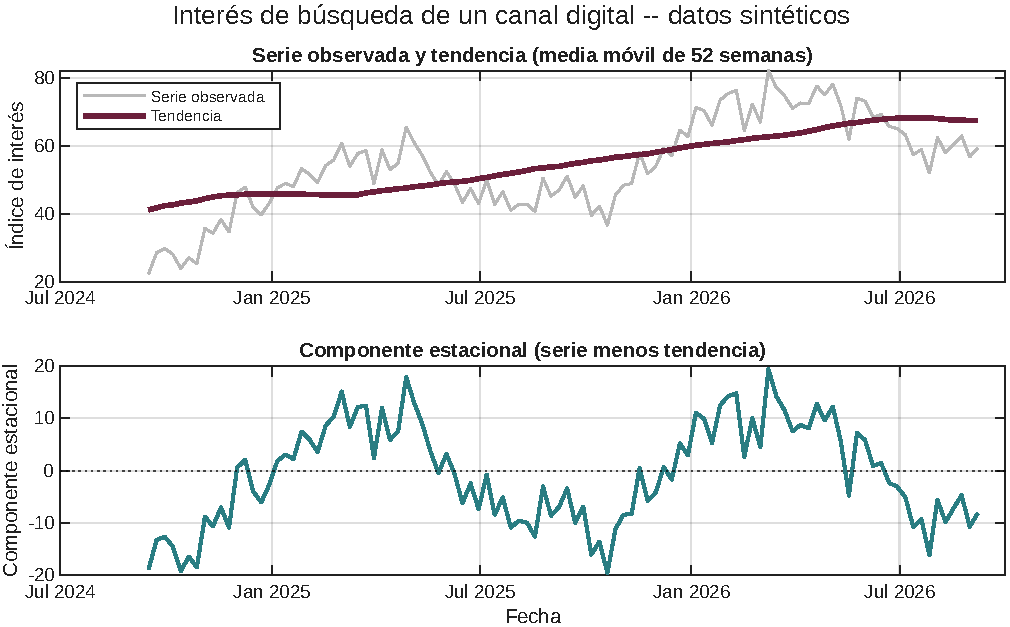
\includegraphics[width=0.95\textwidth]{figuras/matlab/cap04_tendencia_estacionalidad.pdf}
  \captionof{figure}{Serie de interés de búsqueda: observada, tendencia
  (media móvil de 52 semanas) y componente estacional. Fuente: elaboración
  propia con datos sintéticos, \texttt{rng(42)}.}
  \label{fig:cap04-tendencia}
\end{center}

\begin{center}
  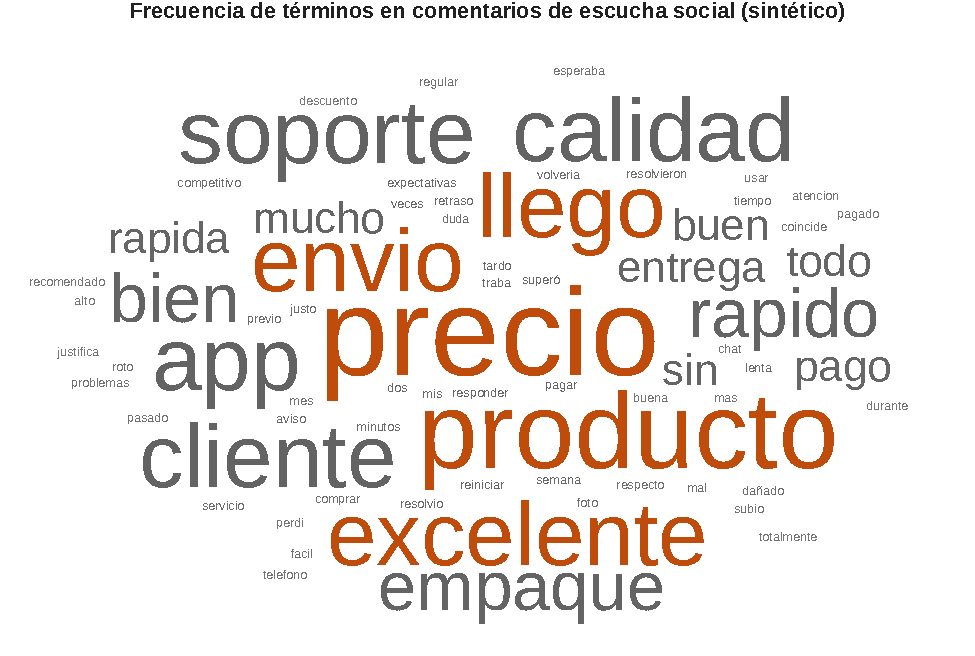
\includegraphics[width=0.72\textwidth]{figuras/matlab/cap04_nube_palabras.pdf}
  \captionof{figure}{Frecuencia de términos en un corpus sintético de
  escucha social. Fuente: elaboración propia con datos sintéticos.}
  \label{fig:cap04-nube}
\end{center}

\textbf{Interpretación de negocio.} El componente estacional de la
figura~\ref{fig:cap04-tendencia} (panel inferior) revela un patrón que la
serie observada (panel superior, línea gris) oculta a simple vista bajo el
ruido semana a semana: un pico recurrente hacia fin de año, de magnitud
similar en ambos ciclos anuales capturados. Una organización que planee
inventario, personal de soporte o presupuesto publicitario a partir de la
serie observada sin aislar este componente corre el riesgo de interpretar
como \enquote{tendencia acelerada} lo que en realidad es la fase ascendente
predecible del ciclo estacional —error que se repite cada fin de año en
organizaciones que no separan ambos componentes—. En la nube de palabras
(figura~\ref{fig:cap04-nube}), los términos dominantes —\textit{precio},
\textit{producto}, \textit{envío}, \textit{llegó}, \textit{excelente},
\textit{soporte}— mezclan menciones positivas y de fricción operativa a
simple vista indistinguibles por tamaño; el ejercicio propuesto pide separar
ambas.

\textbf{Ejercicio propuesto.} Clasificar a mano los diez términos más
frecuentes del corpus en \enquote{asociado a experiencia positiva},
\enquote{asociado a fricción operativa} o \enquote{neutro/descriptivo}, y
discutir si la nube de palabras, por sí sola, sin ese trabajo manual de
clasificación, es una herramienta de análisis o solo de exploración inicial.

\textbf{Extensión opcional.} Sustituir la media móvil de 52 semanas por la
función \texttt{trenddecomp} o \texttt{decompose} disponible en el toolbox
de Econometría (si está instalado) y comparar el componente de tendencia
resultante contra el de este script.
\end{cajaLaboratorio}

\begin{cajaEtica}
Un corpus de escucha social real —a diferencia del sintético de este
laboratorio— contiene texto escrito por personas identificables o
potencialmente identificables. Analizarlo, incluso de forma agregada,
implica las mismas obligaciones de base legal revisadas en el Cap.~3: la
escucha social no está exenta de la LFPDPPP solo porque los comentarios sean
públicos. Publicar públicamente una opinión no equivale a otorgar
consentimiento ilimitado para cualquier uso analítico posterior de esa
opinión.
\end{cajaEtica}

\section{Estudio de caso}

\begin{casoFicticio}
El equipo de mercadotecnia de una marca de electrodomésticos mexicana
observa que su índice de interés de búsqueda de marca subió 20 puntos en
las últimas cuatro semanas y concluye que una campaña reciente de influencer
marketing está funcionando muy bien, con la intención de duplicar el
presupuesto de inmediato. Al revisar el histórico de dos años de la serie
—no solo las últimas cuatro semanas—, un analista nota que el mismo salto de
aproximadamente 20 puntos ocurrió en la misma época del año anterior, sin
ninguna campaña de influencers en curso en ese momento.

\textbf{Preguntas guía.}
\begin{enumerate}
  \item ¿Qué componente de la serie de tiempo (tendencia o estacionalidad)
  explica mejor el patrón que encontró el analista?
  \item Diseñe, en términos generales, cómo el equipo podría aislar el
  efecto real de la campaña de influencers del efecto estacional, usando el
  mismo enfoque de descomposición del laboratorio.
  \item ¿Qué consecuencia de negocio tendría duplicar el presupuesto de una
  campaña basándose en una lectura de la serie que confunde estacionalidad
  con efecto de campaña?
  \item Relacione este caso con la advertencia del caso de apertura sobre
  cifras puntuales de adopción tecnológica: ¿qué tienen en común el error de
  Gartner con el 25\,\% de caída de búsqueda y el error del equipo de
  mercadotecnia de este caso?
\end{enumerate}
\end{casoFicticio}

\section{Actividades y evidencias del portafolio}

\begin{description}
  \item[Reporte de indagación documental] Aplicar la matriz de cuatro
  criterios (cuadro~\ref{tab:cap04-criterios}) a dos plataformas digitales
  vigentes elegidas por el equipo, con al menos una fuente por criterio.
  \item[Exposición] Presentar el hallazgo del componente estacional del
  laboratorio (§3) y proponer una decisión de negocio distinta según se
  ignore o se considere ese componente.
  \item[Solución de casos] Resolver el estudio de caso de la marca de
  electrodomésticos (§4) por escrito.
  \item[Reporte de práctica] Consolidar, junto con los reportes de práctica
  de los capítulos 1--3, el entregable único de la práctica oficial \enquote{El
  consumidor digital y su perfil} (ver \enquote{Prácticas oficiales de la
  unidad} al cierre de esta Parte).
\end{description}

\section{Ruta de aprendizaje autónomo}

Una hora de aprendizaje autónomo. Tarea concreta:
\begin{enumerate}
  \item Investigar, con fecha de consulta registrada, si el estado del
  comercio agéntico descrito en el recuadro de Frontera de este capítulo
  (§2.1) cambió de forma relevante desde la fecha de cierre de este libro
  (18 de septiembre de 2026), y documentar la fuente.
\end{enumerate}

\section{Síntesis}

La base tecnológica del consumidor digital cambia más rápido que cualquier
libro de texto puede documentar con precisión permanente —el propio caso de
apertura de este capítulo lo demuestra con dos predicciones recientes que no
se cumplieron como se anunciaron—. La respuesta pedagógica correcta no es
memorizar el estado actual de las plataformas, sino dominar los criterios
que permiten evaluar cualquier plataforma, presente o futura: modelo de
negocio, intermediación de datos, interoperabilidad y exposición
regulatoria. Analíticamente, dos herramientas recorren todo el capítulo:
separar tendencia de estacionalidad en una serie de tiempo, y extraer
frecuencia de términos de un corpus de texto —ambas, técnicas que siguen
siendo válidas sin importar qué plataforma específica las alimente de
datos.

\subsection*{Glosario del capítulo}
\begin{description}
  \item[Bolsa de palabras (\textit{bag of words})] Representación de un
  corpus de texto como matriz de frecuencias de términos por documento.
  \item[Comercio agéntico] Comercio mediado por asistentes de compra basados
  en inteligencia artificial que buscan, comparan y en ocasiones ejecutan
  transacciones en nombre del consumidor.
  \item[Componente estacional] Patrón que se repite con periodicidad fija en
  una serie de tiempo (p.\,ej., anual).
  \item[Tendencia] Componente de cambio de largo plazo de una serie de
  tiempo, aislado del ruido de corto plazo y del patrón estacional.
\end{description}

\subsection*{Autoevaluación}

\textbf{Opción múltiple}

\begin{enumerate}
  \item El capítulo propone evaluar plataformas digitales con una matriz de
  criterios durables en vez de un catálogo de herramientas porque:
  \begin{enumerate}
    \item[a)] Las herramientas actuales son todas de mala calidad.
    \item[b)] Un catálogo de marcas concretas envejece más rápido que los criterios estructurales que las evalúan. \textit{(correcta)}
    \item[c)] El programa oficial prohíbe mencionar marcas.
    \item[d)] Las plataformas no tienen modelos de negocio distintos entre sí.
  \end{enumerate}
  \textit{Justificación:} §2.1.

  \item En la descomposición de una serie de tiempo, el componente
  estacional se obtiene, en el script del laboratorio, como:
  \begin{enumerate}
    \item[a)] La serie observada multiplicada por dos.
    \item[b)] La serie observada menos la tendencia estimada. \textit{(correcta)}
    \item[c)] El promedio simple de toda la serie.
    \item[d)] La frecuencia de términos del corpus de texto.
  \end{enumerate}
  \textit{Justificación:} §3, concepto detrás del código.
\end{enumerate}

\textbf{Preguntas abiertas}

\begin{enumerate}
  \item Explique por qué el capítulo no reporta cifras de cuota de mercado
  de buscadores ni de tamaño del comercio agéntico como datos verificados.
  \textit{Clave:} la respuesta debe señalar que las fuentes disponibles
  (blogs de industria, analistas) son de jerarquía baja y con frecuencia se
  contradicen entre sí, y que la regla de verificación de datos del proyecto
  exige no reportar como dato duro lo que no se puede confirmar en fuente
  primaria (§3 de este capítulo, \texttt{docs/verificacion-datos.md}).
  \item Con base en el caso de apertura y el estudio de caso del capítulo,
  explique en sus propias palabras el riesgo de tomar decisiones de negocio
  a partir de una serie de tiempo sin separar tendencia, estacionalidad y
  ruido. \textit{Clave:} la respuesta debe identificar que confundir un
  patrón estacional recurrente con un efecto causal específico (una campaña,
  una predicción de mercado) lleva a decisiones de inversión mal
  fundamentadas, replicables en ambos casos presentados en el capítulo.
\end{enumerate}

\section{Lecturas recomendadas}

\begin{description}
  \item[\textcite{eprs2025darkpatterns}] Aunque centrado en patrones oscuros
  (desarrollado con detalle en el Cap. 7), este informe del Parlamento
  Europeo ofrece un panorama actualizado de regulación digital útil para el
  criterio de \enquote{exposición regulatoria} de la matriz de este
  capítulo.
  \item[\textcite{sheth2026}] Su enfoque de organizar el comportamiento
  digital por mecanismos de datos, más que por plataformas específicas, es
  coherente con el criterio metodológico que este capítulo propone para
  evaluar la base tecnológica.
\end{description}
